\documentclass[11.5pt]{article}

\usepackage{amssymb, amsmath, amsthm, amsfonts, eurosym, geometry, ulem, graphicx, caption, color, setspace, footmisc, pdflscape, array, todonotes, subfig, adjustbox, booktabs, pdfpages, siunitx, setspace, multirow, tikz, appendix}

\usepackage[flushleft]{threeparttable}
%\usepackage{hyperref}
\usepackage{natbib}
\bibliographystyle{plainnat}
%\usepackage[round]{natbib}
\usepackage[applemac]{inputenc}
\usepackage{hyperref}
%\usepackage{xcolor}
%\hypersetup{
%  colorlinks   = true, %Colours links instead of ugly boxes
%  urlcolor     = red, %Colour for external hyperlinks
%  linkcolor    = blue, %Colour of internal links
%  citecolor   = blue %Colour of citations
%}

\geometry{left=1in,right=1in,top=1in,bottom=1in}

\captionsetup{justification=justified}

\setlength{\textwidth}{6in}
\setlength{\oddsidemargin}{.22in}
\setlength{\textheight}{9in}
\setlength{\topmargin}{-0.10in}
\setlength{\headheight}{0.02in}

\normalem

\onehalfspacing
\newtheorem{theorem}{Theorem}
\newtheorem{corollary}[theorem]{Corollary}
\newtheorem{proposition}{Proposition}

\newtheorem{conjecture}{Conjecture}
\newtheorem{example}{Example}
\newtheorem{definition}{Definition}
\newtheorem{assumption}{Assumption}
\newtheorem{remark}{Remark}

%\newenvironment{proof}[1][Proof]{\noindent\textbf{#1.} }{\ \rule{0.5em}{0.5em}}

\newtheorem{hyp}{Hypothesis}
\newtheorem{subhyp}{Hypothesis}[hyp]
\renewcommand{\thesubhyp}{\thehyp\alph{subhyp}}

\newcommand{\red}[1]{{\color{red} #1}}
\newcommand{\blue}[1]{{\color{blue} #1}}

\newcolumntype{L}[1]{>{\raggedright\let\newline\\arraybackslash\hspace{0pt}}m{#1}}
\newcolumntype{C}[1]{>{\centering\let\newline\\arraybackslash\hspace{0pt}}m{#1}}
\newcolumntype{R}[1]{>{\raggedleft\let\newline\\arraybackslash\hspace{0pt}}m{#1}}

\geometry{left=1.0in,right=1.0in,top=1.0in,bottom=1.0in}

\captionsetup{justification=justified}
\renewcommand{\baselinestretch}{1.3}
\newcounter{marginparcounter}
\newcommand{\patopar}[1]{\stepcounter{marginparcounter}$^{(\roman{marginparcounter})}$\marginpar{\color{red}\renewcommand{\baselinestretch}{0.8}\scriptsize$^{(\roman{marginparcounter})}$ PD: #1}}
\renewcommand{\baselinestretch}{1.3}
\setlength{\textwidth}{6in}
\setlength{\oddsidemargin}{.22in}
\setlength{\textheight}{9in}
\setlength{\topmargin}{-0.10in}
\setlength{\headheight}{0.02in}
%\setlength{\parskip}{0.4cm}

\renewcommand{\thesection}{\Roman{section}}
\renewcommand{\thesubsection}{\Alph{subsection}}

\newcommand{\appendixpagenumbering}{
  \break
  \pagenumbering{arabic}
  \renewcommand{\thepage}{\thesection-\arabic{page}}
}

% ---------------------------------------------------------------------------------------
% ---------------------------------------------------------------------------------------

\begin{document}
% Multidimensional Aspirations: \\ Experimental Evidence of Micro-entrepreneurs' Aspirations for Child Education and Business Growth
\title{\Large \textbf{Shocking Aspirations: \\Experimental Evidence for the Effect of Aspirations on Small-business Growth in Indonesia}\thanks {\scriptsize We thank the Abdul Latif Jameel Poverty Action Lab (J-PAL) for hosting our study, in particular Raisa Annisa, Ni Luh Putu Satyaning Pradnya Paramita, Lukman Edwindra, and Dwitri Amalia for excellent research assistance. This paper was produced under the framework of the \textquotedblleft Enabling Innovation and Productivity Growth in Low Income Countries (EIP-LIC/PO5639)" project, funded by the Department for International Development (DFID) of the United Kingdom and implemented by Tilburg University. Additional funding was received by The World Bank. Research on the ground was conducted in cooperation with J-PAL South-East Asia and SurveyMETER.}}

\author{Patricio S. Dalton\thanks{\scriptsize Tilburg University, Department of Economics and CentER, Warandelaan 2, 5037 AB, Tilburg, The Netherlands. E-mail corresponding author: \texttt{p.s.dalton@uvt.nl} (corresponding author), \texttt{j.ruschenpohler@uvt.nl}}
\and Julius R\"uschenp\"ohler\footnotemark[2]
\and Bilal Zia\thanks{\scriptsize The World Bank, Development Research Group, 1818 H St. N.W. Washington, D.C. 20433. E-mail: \texttt{bzia@worldbank.org}.}}


\date{\today}
\maketitle
\singlespace

\begin{abstract}
\noindent {In a randomized controlled trial in Jakarta, Indonesia, we open the aspirations windows of small-scale entrepreneurs and measure the effects on business and family aspirations, business performance, and subjective well-being. We develop handbooks on business practices that are locally profitable and come at essentially zero economic costs to provide an informational shock to entrepreneurial aspirations. In order to identify specific channels to increase aspirations, we administer two additional treatments. First, we select five role models on the local frontier of best practices and expose a subset of entrepreneurs to their example to facilitate social learning. Second, we provide personalized, hands-on implementation assistance to another subset of entrepreneurs to foster adoption through first-hand learning. In line with the theoretical literature, we find pronounced heterogeneous treatment effects that differ by baseline levels of aspirations. Six months after treatment, entrepreneurs who aspired high at baseline, have increased their aspirations, and earn markedly higher business sales and profits. [INCL NUMBERS] %Interestingly, this heterogeneity arises after both the movie treatment and the assistance. 
In contrast, those with low initial aspirations see their aspirations and performance decrease by roughly the same amount. [INCL NUMBERS] 18 months after treatment, effects grow only more pronounced. We confirm the same heterogeneity in the entrepreneur's aspirations for their children's education and their reported satisfaction with household finances. This suggests that, in the absence of binding economic constraints, aspirations windows can be opened with locally relevant low-cost interventions and that their effect on aspirations and business growth hinges on the individual's distance to the frontier.}\\



\noindent\textbf{Keywords:} Aspirations, aspirations failure, aspirations frustration, small-business growth, business performance, subjective well-being, randomized controlled trial, field experiment.\\
\noindent\textbf{JEL Codes:};
\end{abstract}
\vfill

\thispagestyle{empty}

\pagebreak

\onehalfspacing

\setcounter{page}{1}


\section{\textbf{Introduction}}

It is a long-standing puzzle in development economics why poor individuals and small-scale businesses often do not exploit what have been shown to be propitious investment opportunities (see, e.g., de Mel et al, 2008). Beyond classical work on imperfections in the markets for credit and insurance (e.g., Banerjee et al., 2015), a lack of formal saving instruments (e.g., Dupas and Robinson, 2013a,b), or institutional constraints (e.g., Bardhan, 1997), a more recent literature points towards psychological constraints as a possible explanation for foregone investments both on the individual and on the firm-level (see, e.g., Duflo, 2012; Bernheim et al., 2015; Banerjee and Mullainathan, 2008). As part of this literature, Appadurai (2004) and Ray (2006) have argued that poverty may affect the individual's capacity to aspire and thus hamper their ability to contest their poverty. In their view, aspirations are, in part, socially determined by the agent's aspirations window, comprising the achievements of spatially, economically, and socially similar others. Dalton et al. (2016) develop a framework in which poverty exacerbates existing cognitive biases creating a behavioral poverty trap in which suboptimally low levels of aspirations and investment reinforce each other to yield ever lower levels of achievement. Policies which exogenously shock aspirations can help the poor escape a poverty trap, provided that initial aspiration levels are not too low and that resources to satisfy aspirations are available. Galiani et al. (2018) extend this by showing how changes in aspirations may be short-lived if resource constraints are binding.

In this paper, we provide experimental evidence for how, in a realistic case without binding constraints in economic resources, aspirations affect business growth. In a randomized-controlled trial (RCT) among small-scale entrepreneurs in the traditional retail sector of Jakarta, Indonesia, we experimentally test the malleability of business aspirations by providing exogenous change to entrepreneurs' aspirations windows. We measure the causal impact of this change in aspirations on business performance and further investigate the effects on the entrepreneur's aspirations towards their children's education. In order to further identify specific channels in increasing aspirations, we distinguish four different interventions. First, we combine the results from an extensive baseline survey on locally profitable business practices with qualitative interviews on implementation practices to develop a handbook of local best practices (hereafter \emph{Handbook}) which we distribute to all 1040 treated entrepreneurs. We interpret the \emph{Handbook} as a pure shock to the information available to the entrepreneur on pathways to business growth. Crucially, practices are adapted to the background in suitability and simplicity and come with all physical resources necessary such that the economic costs of adoption are essentially zero. Second, based on these qualitative interviews, we select five successful role models to relate their implementation advice through a documentary (hereafter \emph{Movie}) which we invite a random subgroup of 520 business owners to watch in public screening events. Exposure to the \emph{Movie} exogenously varies the extent to which entrepreneurs can engage in social learning from role models who embody the usefulness of the set of practices outlined in the \emph{Handbook}. Third, we use both data sources further to design an intervention in which trained local staff provides a subgroup of 520 entrepreneurs with two sessions of personalized, hands-on implementation assistance on topics of the handbook (hereafter \emph{Assistance}). The \emph{Assistance} varies the extent to which entrepreneurs can engage in practical first-hand learning. This is designed to foster adoption by convincing the entrepreneur of the applicability of the practices in their idiosyncratic environment. Fourth, 260 entrepreneurs are randomly selected to receive a combination of \emph{Movie} and \emph{Assistance} alongside the \emph{Handbook} to test for possible complementarities. We estimate treatment impacts vis-\`{a}-vis a control group 261 entrepreneurs (hereafter \emph{Control}) six and 18 months after treatment.

Since we expose all entrepreneurs to the same frontier of practices, change in aspirations windows at the individual level should differ by the distance of the entrepreneur's aspirations to the frontier. We exploit this variation in treatment shocks to estimate the heterogeneity in effects for subgroups whose business aspirations are high (closer to the frontier) versus low (further from the frontier) at baseline. Business owners with high initial aspiration levels should benefit most from a widening of their aspirations windows, be it through a pure information shock or entrepreneurial role models. On the contrary, and in line with Ray (2006) and Genicot and Ray (2017), entrepreneurs too far from the frontier may initially engage with the practices but soon see their aspirations frustrated. 

Six months after treatment, we find statistically significant and economically meaningful effects on several dimensions of business aspirations as well as on business sales and profits. These effects grow only more pronounced after 18 months. In particular, entrepreneurs whose business aspirations are above the median at baseline increase their aspirations in reaction to both \emph{Movie} and \emph{Assistance} and show considerable gains in business sales and profits. [INCL. NUMBERS] In contrast, and in line with aspirations frustration (Ray, 2006; Genicot and Ray, 2017), we find that entrepreneurs who report below-median aspirations at baseline lower their aspirations further and report reductions in business performance. [INCL NUMBERS] We show that this pronounced heterogeneity for subgroups differing in baseline levels of business aspirations is also reflected in the entrepreneur's aspirations for their children's education and self-reported levels of financial satisfaction. {INCL NUMBERS]

This paper contributes to three broad strands of literature. First, it adds to the empirical literature on aspirations and poverty (e.g., Bernard et al., 2014; Riley, 2017; Beaman et al., 2012; Janzen etal., 2017). This literature has largely corroborated the view that aspirations correlate with forward-looking behaviour and investment in panel data (see, e.g., Janzen et al., 2017; Dalton et al., 2018; Macours and Vakis, 2014; Kosec and Mo, 2017; Favara, 2017; Ross, 2017; Serneels and Dercon, 2014). While some recent work suggests aspirations may indeed be amenable to change by exposure to role models (see, e.g., Bernard et al., 2014; Macours and Vakis, 2014; Beaman et al., 2012; Riley, 2018), the evidence has been largely confined to educational aspirations. It is unclear whether the same holds for small-scale businesses, a domain of great relevance for the developing world (Maloney 2004; Gollin 2008; Nichter and Goldmark 2009). Further, a key notion of Ray (2006) and Genicot and Ray (2017), that aspirations which far exceed the individual's potential may result in aspirations frustration and lower effort, has been studied only with cross-sectional data (see, e.g., Janzen et al., 2017). In this paper, we provide first experimental evidence both on the impact of a widening in aspirations windows on business aspirations and on business performance. On a more general level, by promoting the use of simple business practices that can be implemented at no monetary cost, we differ from Bernard et al. (2014) and Galiani et al. (2018) in that we show the effects of aspirations in an environment where economic constraints to satisfying higher aspirations are not binding. We add further by investigating the role of psychological resources under these conditions in explaining changes in aspirations and small-business growth. Our results from heterogeneous treatment effects are first experimental confirmation for the theoretical concept of aspirations frustration due to Ray (2006) and Genicot and Ray (2017). Finally, we contribute methodologically in providing a novel approach to measuring aspirations on the essential dimensions of small-business growth.

Second, we contribute to the literature on small-business growth. In Dalton et al. (2018), we document strong associations between business aspirations and forward-looking firm behavior, such as productive investment, loan take-up, and innovation. Here, we complement this aspirations-based view of entrepreneurial behavior with evidence of both the malleability of business aspirations and their impact on firm profitability. This has implications also for strands of this literature which focus on business mentoring (e.g., Brooks et al., 2018; Cai and Szeidl, 2016), business counseling, consulting, and training (for reviews, see Carpena et al., 2017; McKenzie and Woodruff, 2014), and business plan competitions (e.g., McKenzie, 2017; Bjorvatn et al., 2015). Lastly, our findings speak to a recent literature on the identification of businesses with potential for rapid growth (see Fafchamps and Quinn, 2016; Fafchamps and Woodruff, 2017). We provide evidence that exogenous change in aspirations windows does indeed cause business growth. In particular the heterogeneity we find in treatment effects puts emphasis on the study of aspiration levels and provides policy implications as much for the design of interventions as for targeting efforts ex ante.

Third, the paper adds to the growing literature on the effectiveness of role models in promoting behavioral change (see, e.g., Berg and Zia, 2013; Chong and La Ferrara, 2009; Kearney and Levine, 2015; Beaman, et al., 2012; Bernard et al., 2014; Riley, 2017). Emanating from psychology, work on gender stereotypes has shown how exposure to experts and other extraordinary proponents of the same gender  can change stereotypes regarding gender roles and facilitate women's entry into traditionally male industries and roles (e.g., Stout et al., 2011; Asgari et al., 2010). In Economics, interventions involving role models have been used to affect financial knowledge and behaviour (Berg and Zia, 2013), separation and divorce rates (Chong and La Ferrara, 2009), teen pregnancies (Kearney and Levine, 2015), educational outcomes (Beaman et al., 2012; Riley, 2017), or individual investment behavior and savings (Bernard et al., 2014). We add to this in providing evidence that role-model interventions can also affect the growth aspirations of small-business owners and their business performance. We further contribute by quantifying the effect of this intervention against a purely informational shock.

The paper is organized as follows. In Section II, we introduce the concepts of aspirations failure and aspirations windows and lay out our own approach in connection to this literature. We present the data as well as the measurement of key variables in Section III and outline the experimental design and the methods in Section IV. Section V documents the findings which we discuss in Section VI. Section VII concludes.

\section{Aspirations and Investment} \label{sec:hypotheses}

\subsection{Aspirations Failure}

The concept of aspirations and its potential for explaining patterns of persistent poverty is not new to the study of development economics. Dalton et al. (2016) develop a model in which differences in initial wealth exacerbate common behavioral biases to produce an aspirations-based poverty trap. In it, behavioral individuals take their aspiration levels as given when choosing to invest effort, even though aspirations are determined by their effort in equilibrium. For both the poor and the rich, this bias leads to suboptimal choices of effort investments. However, since lower wealth levels reduce the marginal benefit of exerting effort, it is the poor individuals who are more likely to aspire below their true potential. That is, poor individuals optimally choose to exert less effort and to set less ambitious goals with respect to their true potential. This leads to multiple welfare-ranked equilibria. Under the condition that economic constraints are not binding, and depending on initial levels of aspirations, an exogenous shock to aspirations can propel the individual out of the bad equilibrium of an aspirations failure to choose higher aspirations and effort and to achieve better outcomes. Galiani et al. (2018) shed light on the case in which resource constraints are, in fact, binding. Here, the poor individual, once propelled out of the bad equilibrium of a poverty trap through an exogenous shock to aspirations, may not be able to sustain their increased aspirations in the long-term. In the context of a field experiment that randomizes improvements in housing quality to inhabitants of poor slums in Mexico, Uruguay, and El Salvador, the authors show that individuals in the control group indeed report higher aspirations for home improvements in the short-term. On the contrary, investment levels do not change and any gains in aspirations have vanished eight months after treatment. In the presence of resource constraints, aspirations may adapt.

Our paper ties in directly with this literature. We differ from Galiani et al. (2018) in that we offer not only step-by-step guidance on easy to implement and locally relevant business practices but additionally provide any material necessary for the entrepreneur to emulate these practices. That way, we create an environment with essentially zero economic costs to adoption. This is close to Macours and Vakis (2014) who find that, when provided with the necessary resources to follow through on aspired investments, a widening of aspirations windows through exposure to local role models can be sustained beyond the short-term. Furthermore, business models in the retail sector, and particularly among small-scale businesses in the traditional sector, are relatively straight-forward and comparable across businesses. Taken together, we believe this provides us with a realistic case to study the impact of opening aspirations windows on small-business growth when resource constraints are not binding.

\subsection{Aspirations Windows and Aspirations Frustration}

In our approach, we further draw on Ray's (2006) work on the social formation of aspirations. In this view, individuals have aspirations windows which contain "her zone of 'similar', 'attainable' individuals" (Ray, 2003, p.1), that is, their "spatially, economically, perhaps even socially" close others (idem, p.2). Aspirations are formed through "the lives, achievements, or ideals" (idem, p.2) of such individuals. Consistent with this, there is broad empirical support for the notion that relative status within a community or neighborhood has some bearing on individuals' aspirations (Beaman et al., 2012; Janzen et al., 2017; Knight and Gunatilaka, 2012; Fafchamps and Shilpi, 2008; Stutzer, 2004). In an instructive example, Macours and Vakis (2014) show how plausibly exogenous proximity to females in leadership positions may have opened local women's aspirations windows in a field experiment in Nicaragua. 

Inherent in this view of socially determined aspirations is the notion that aspirations may be lifted by opening aspirations windows (see Ray, 2006; Genicot and Ray, 2017; Janzen et al., 2017). Conceptually, aspiration levels are commonly modeled as reference points which affect individual satisfaction derived from achieving a desired goal (see, e.g., Genicot and Ray, 2017; Dalton et al., 2016; Bogliacino and Ortoleva, 2013). In the framework of Genicot and Ray (2017), the agent maximizes the net benefits of effort investment considering two possible outcomes: satisfying their aspirations or failing to satisfy them. Under this scenario, there is a threshold level of aspirations at which the agent is indifferent between exerting high effort and reaping utility from satisfying their aspirations and exerting low effort in frustration. Hence, opening aspirations windows may only be optimal up to a point beyond which individuals in the zone of "similar others" may become too dissimilar to the agent and aspiration levels too high to be worthwhile attaining. In the words of Ray (2003, p.4): "If economic betterment is an important goal, the aspirations window must be opened, for otherwise there is no drive to self-betterment. Yet it should not be open too wide: there is the curse of frustrated aspirations."

By opening aspirations windows up to the same level for all entrepreneurs, we ask whether the distance between the individual's aspiration level and the local frontier can predict potential heterogeneity in treatment effects. Entrepreneurs aspiring high at baseline will be more likely to perceive the shock provided through the \emph{Handbook} as a marginal enlargement of their aspirations window by the achievements of similar others and will react by increasing aspiration levels and expending greater effort. In contrast, entrepreneurs with low aspirations at baseline will see dissimilar others migrate into their aspirations window. As a consequence, these individuals will be more likely to succumb to aspirations failure and will exert less effort. We recognize that purely informational shocks to individuals' aspirations windows may not be sufficient to spur additional effort. That is, in the absence of  economic constraints, psychological constraints to satisfying aspirations may still be present. Hence, in a second step, we test the impact of two kinds of complementary psychological resources that go along with the \emph{Handbook}. First, the \emph{Movie} provides a personal experience with selected entrepreneurs, presented as "similar" but successful others. This intervention is aimed at convincing the entrepreneur of the similarity shared between them and provides an opportunity to learn through the actual achievements of a role model rather than to engage with the same set of practices in a purely informational way. Since we designed the advice captured in the \emph{Movie} to be almost perfectly identical with the content of the \emph{Handbook}, any differences between treatment groups are unlikely to be caused by a pure information shock. On the other hand, it is also conceivable that the \emph{Handbook} has limited impact on effort and performance since it makes entrepreneurs engage with material they may construe as being too dissimilar to their own skill set as to engage with it productively. The \emph{Assistance} is designed to remedy this constraint by providing personalized, hands-on assistance which may convince entrepreneurs of the applicability of the selected practices to their own idiosyncratic environment beyond what an informational shock can deliver.

\section{\textbf{Data}}


\subsection{Study Location and Population of Interest}

The field work for the study was conducted in Jakarta, the capital city of Indonesia. While the city of Jakarta is home to roughly 10 million inhabitants, 30 million people live in its metropolitan area including the peripheral cities of Bogor, Depok, Tangerang, and Bekasi (``Jabodetabek''). We draw our sample from the population of traditional retail businesses in the city of Jakarta (excluding ``Jabodetabek''). Locally known as ``toko kelontong'' or ``warung'', shops of this kind are ubiquitous in Indonesia where retail and hospitality is the second largest sector of MSE employment following agriculture (Kementerian Koperasi dan UMKM, 2011). Offering staples such as rice, nuts, and beans but also snacks, sweets, beverages, toiletries, cigarettes, and other convenience goods, traditional retail shops are concentrated largely in residential areas and adjacent to traditional markets for vegetables, fruits, rice, meat, and fish. Most are operated as family businesses with only 2.43\% employing any hired labor. Appendix \ref{sec:expbusinesses} shows pictures of two shops representative of this sample.


\subsection{Sampling Frame}

For logistical reasons, we restricted the area of study to the 144 districts of the city of Jakarta, excluding the wider metropolitan area (``Jabodetabek''). Of the 144 districts that comprise the city of Jakarta, we dropped all 32 districts of Northern Jakarta (``Kota Jakarta Utara'') due to an SME training program concomitantly run by a large retail chain. Out of the 112 eligible districts, we randomly selected 29 districts to be part of the research.\footnote{Appendix \ref{sec:maps} provides a map of the districts of study in the context of the wider metropolitan area.} Within these 29 areas of study, we conducted a listing exercise to create a list of all businesses which met the following five selection criteria: (1) shop size of at least $4m^2$, (2) at least two different product categories on offer, (3) a general interest of the entrepreneur to see their business grow, (4) no handcart or other moveable business premises, and (5) no franchise of larger retail chains. Regarding the sampling procedure, within each district a team of two to three enumerators would first request a map of \textit{community-level} boundaries at the local district office. This enabled us to avoid market places whose high population density would make the research design vulnerable to spill-over concerns. We further aim to avoid spill-overs by sampling only businesses which were at a distance of at least 30 meters. This procedure yielded a total of 2042 businesses of which we randomly selected a sample of 1301 to be included in the study.

\subsection{Measurement of Variables}

The empirical analysis of this paper draws on two waves of a business survey with a baseline conducted in March and April 2016 and an endline fielded in October and November 2016. Besides a wide range of entrepreneurial and business characteristics, this survey included detailed measures on the aspirations of the entrepreneur. In this regard, we measure both business aspirations and aspirations towards the education of the entrepreneur's children. Lastly, the survey includes questions on the satisfaction of the entrepreneur with their financial situation and life in general.

Regarding business aspirations, we elicit both short-term and long-term aspirations for different dimensions of the business. For the short-term, we ask we ask: ``Please imagine your business a year from now. How large do you imagine your business premises to be? How many people will work there? How many customers will come by on a normal day? What are the daily sales you aspire to have?''. For the long-term, we ask ``\emph{Please imagine your ideal business. How large is your shop? How many people work there? How many customers come by on a normal day?}''. Complementing these long-term aspirations, we elicit the aspirations horizon: ``\emph{How many years do you think it will take for you to achieve your ideal business?}''. On each dimension, responses are primed by reminding respondents of their current levels. Respondents answer with estimates in square meters, numbers of employees and customers, and amounts of daily sales in Indonesian Rupiah. We use the levels for each dimension as outcomes to capture potential treatment effects. Additionally, we compute aggregate scores for business aspirations by averaging z-scores of each dimension in the short-term and in the long-term, respectively.

Further, we measure the aspirations of the entrepreneur towards their son's and daughter's educational attainment. For this, we first record the respondent's offspring by asking: ``Do you have any sons [daughters] and, if so, what are their names and how old are they?''. We then elicit aspirations regarding the oldest son and the oldest daughter under the age of 18, respectively. Specifically, we ask: ``How many years of schooling do you aspire him [her] to achieve?''. Respondents answer with estimates in years or are aided by the enumerator in translating any degree to the number of years necessary to acquire it in the Indonesian education system. We use the number of years as an outcome and construct a dummy variable that takes on the value one if the entrepreneur aspires for their son [daughter] to acquire at least Master's level education and zero otherwise.

The entrepreneur's subjective well-being is proxied by their overall satisfaction with household finances and life in general at the time of the survey. We use standardized questions from the World Values Survey and ask: How satisfied are you with the financial situation of your household?'' and ``How satisfied are you with your life at this point?''. Respondents are instructed to answer on a scale from one to ten, whereby one indicates ``very dissatisfied'' and ten indicates ``very satisfied''.


\subsection{Summary Statistics}

Table \ref{XXX} presents summary statistics on owner background characteristics, business characteristics, as well as business and educational aspirations from baseline data. Column (1) shows means and standard deviations of the full sample of 1301 businesses. Columns (2) to (6) present the means for businesses assigned to each of the experimental groups, respectively.

The median entrepreneur in this sample is female (70.83\%), 45 years of age, and has completed 9 years of formal education or the equivalent of middle school ($mean = 9.39$ years). However, this masks considerable heterogeneity as 46.78\% have finished high-school and 4.44\% hold college degrees. At the time of the baseline survey, the median business has been operative for 10 years. It has two workers, measures ten square meters in size, and sees a total of 40 customers on a typical day. Median monthly profits are USD 370.17 PPP ($mean = 477.45$) with median monthly sales of USD 2961.35 PPP ($mean = 6034.93$). Within 12 months from the baseline survey, the median business owner aspires to daily sales on the order of USD 246.78 PPP. They further report aspirations for business growth to 12 square meters in size ($mean = 15.56$) but for no change in the number of employees ($mean = 1.72$) and the number of customers ($mean = 56.85$). In addition, we elicit long-run aspirations for the imagined ideal business, which the median entrepreneur estimates to be achieved in 2 years ($mean = 2.77$). In the long-run, the median shop owner aspires to a business of 16 square meters in size ($mean = 24.19$) with a total of 50 daily customers ($mean = 73.35$). Aspirations for employment growth are no higher than current levels ($mean = 2.09$). Regarding their children's prospects, aspirations exceed the educational attainment of the entrepreneur by a considerable margin. The median business owner aspires for their child to complete 16 years of schooling ($mean = 16.81$) while 27\% aspire to Master's-level education for their offspring. %In terms of occupational prospects, most entrepreneurs aspire their children to work in government offices on the local, regional, or national level or as publicly employed teachers (63.41\%).

Table \ref{XXX} presents balance checks for the baseline sample. Columns (5) to (7) present p-values for differences-in-means tests between the three groups. The table shows that the randomization was successful. Out of 64 difference in means tests performed, only 3 return statistically significant differences, which would be expected in random sampling.

\subsection{Survey Attrition}

We document two sources of attrition among respondents: (1) owners of shops which close down and cannot be tracked and (2) owners who refuse to take part in the endline survey. Regarding its effect on statistical power, attrition levels are low. At endline, we document a loss of about 8\% of the overall sample. This places our study at the lower end of the distribution of business training interventions in developing countries for which attrition rates are typically in excess of 10\% and can reah up to 25\% or higher (for a review, see McKenzie and Woodruff, 2014). In fact, attrition is in line with commonly observed levels in household panel surveys (Hill, 2004).

Moreover, the event of whether a respondent attrits or not is not correlated with treatment status. Table \ref{XXX} presents regression analyses of survey attrition on treatment status. Columns (1) and (2) presents results for differential attrition due to respondents refusing the endline interview. Columns (3) and (4) show the same analysis for attrition due to closures. Even-numbered columns report regression models with added stratification controls.


\section{\textbf{Experimental Design and Methods}}

\subsection{Experimental Design}

In order to create exogenous variation in the exposure to treatment, we divided the full sample of 1301 businesses into four treatment groups ($N = 260$ each) and one control group ($N = 261$). Randomization was stratified according to (1) gender, (2) business size (below 6$m^2$, between 6 and 10$m^2$, or above 10$m^2$), and (3) a dummy of whether the entrepreneur scored above or below the median in a composite of business practices.

Each of the treated individuals ($N = 1040$) received the \emph{Handbook} which characterized local best practices in doing business and provided step-by-step advice on their implementation. Orthogonal to this treatment, a random subset of shop owners ($N = 520$) was invited to the screening of the \emph{Movie} which featured the success stories of five local entrepreneurs. A second subset of shop owners ($N = 520$) received an invitation to \emph{Assistance}, two sessions of personalized business assistance which were based on the content of the handbook and were designed to clear up misunderstandings and aid with implementation issues. A cross-design ensured that 260 participants received the \emph{Handbook Only}, while other 260 participants were assigned to each of three additional groups: \emph{Handbook and Movie} ($N = 260$), \emph{Handbook and Assistance} ($N = 260$), and \emph{All Three} treatments ($N = 260$).

Regarding the timing of activities, we conducted the listing exercise in January 2016 and administered the baseline survey in March and April 2016. Interventions took place in October and November 2016. These were followed by a first endline survey conducted in April and May 2017 and a second endline survey in April and May 2018.\footnote{For a detailed timeline, see Appendix \ref{X}.}

\subsection{Interventions}

\subsubsection{Handbook}

\emph{\textbf{Selection of Best Practices}}\

The business practices presented in the \emph{Handbook} are those found to be most profitable in the local context among a total set of 84 practices tested. In order to identify these local best practices, we rely on data from qualitative interviews with 102 small-scale entrepreneurs and from the quantitative baseline survey conducted among all 1301 business owners included in the study sample. The process is described in more detail in Dalton et al. (2018b). Importantly, we use the qualitative data to inform implementation advice in both the \emph{Handbook} and \emph{Assistance} intervention. The quantitative baseline data is used to estimate the returns to adoption of each practice and ultimately to select the set of best practices. We use multivariate regression models to regress firm performance measures, such as the number of daily customers and different measures of business sales and profits, on business practices. The set of best practices is selected according to two criteria: 1) the practice's significance in predicting firm performance measures across eight different OLS specifications and 2) the absolute value of the effect on performance. That way, we are able to reduce the total set of 84 practices to 14 most profitable practices. We subsequently 2 marketing practices, 3 in stocking-up, 4 in record-keeping and profit calculation, 1 in financial planning, and 3 in discussing and cooperating on business matters. 

Appendix \ref{sec:selprac} provides a list of all practices mentioned in the handbook. Besides the set of 14 best practices, additional practices were mentioned in the handbook. These practices served mainly as entry points to the narrative of a chapter or as connecting points between two or more selected practices. While we provide information on the estimated returns to adoption on all selected practices, we show no such information for this set of accessory questions. \\

\noindent \emph{\textbf{Handbook Production}}\

The \emph{Handbook} is designed to introduce the set of local best practices identified through the baseline data and to provide both reasons to adopt the practices and a clear guide to implementation. We grouped the selected practices in five semantic groups: keeping records, calculating profits, planning stock-up purchases, attracting new and retaining old customers, and discussing and cooperating on business decisions. One chapter of approximately 10 to 15 pages was devoted to each of the semantic groups. In each chapter, we address major misconceptions which we found entrepreneurs use to rationalize non-adoption or procrastination on adoption decisions in the qualitative interviews. We highlight returns to adoption information of each of the selected practices and outline simple implementation strategies which embed each practice into the broader narrative of the chapter. %For instance, in the case of record-keeping (chapter 1), the reader first learns to separate accounts before they are introduced, step by step, to building a structured account of every business transaction that takes place. This leads up to practical ways to calculate profits at the end of the chapter. Along the way, the entrepreneur learns to deal with common situations, such as how to note down the event of lending money to one's friends and family and how to document any event of extending trade credit. 
Each chapter ends with a number of tips for the advanced user, such as applying for a token-based electricity meter which helps keep costs in check and aids keeping account of the costs. %In order to enable the reader to not only read cover to cover but also more cursorily, all chapters are self-contained and each section within a chapter provides links to other points in the chapter which explain background knowledge in more detail. 
A cheat sheet of 12 pages complements the \emph{Handbook} to summarize the main information in condensed form. An additional exercise book is meant to minimise transactions costs of adoption and enables the reader to start practicing the structure conveyed in the \emph{Handbook} regarding both record-keeping and stock-up planning right away.

\subsubsection{Movie}

\emph{\textbf{Selection of Role Models}}\

\noindent In order to identify potential entrepreneurs whose businesses were comparable to those of the sample in type but distinct in the level of organization, growth aspirations, practices, and size, we used the qualitative data on 102 shop owners to create a list of nine candidates. Short-listed candidates were entrepreneurs who used the greatest number of business practices as measured by the battery provided by McKenzie2017. In-depth interviews with these candidates were conducted to reveal their aspirations for business growth and history as small-scale retailers. Further, we enquired into business practices used and encouraged the candidates to elaborate on personal experiences and to give advice crucial for implementation. Based on these interviews, we selected five entrepreneurs who best represented the local frontier of best practices and acquired informed consent for their appearance as role models in our \emph{Movie}.

The final sample of entrepreneurial role models are heterogeneous in socio-demographics, such as gender, age, and ethnicity, and own businesses disparate in size. Drawing on the anthropological and psychological literature on social learning, we use this heterogeneity to ensure similarity with the greatest possible fraction of the sample tapping into individuals' tendency to learn from similar others (Chudek et al., 2013; Corriveau and Harris, 2009; Efferson et al., 2008; McElreath et al., 2008; Morgan et al., 2011; Rendell et al., 2011). Moreover, the difference in business size is intended to show the range of possibilities for a business of the same type as those in the sample and thus to facilitate the opening of ``aspirations windows'' (Ray, 2006). On average, the largest shops in our sample are larger than the smaller role-model businesses but smaller than the largest. Smaller shops in our sample are as small as the very smallest role-model business.\\

\noindent \emph{\textbf{Movie Production}}\

\noindent A professional production company was hired to conduct both the shooting of the \emph{Movie} and the post-production editing. The research team was in charge of every aspect pertaining to the content of the film. As such, we wrote a script which comprised the full set of questions that would be asked and distributed it days before the shooting started to ensure informed consent on the part of the participants. The final \emph{Movie} is 25 minutes in length and portrays the five selected role models, their advice and businesses. Each entrepreneur is prompted to elaborate on their use of a set of related practices, the impact of their use on the business, and specific implementation advice. The set of practices presented by each role model roughly corresponds to one chapter in the \emph{Handbook}. Moreover, entrepreneurs are asked about their past as small-scale retailers and about their aspirations for future growth. In sum, through each role model, aspirational goals are established and business practices presented which are framed as pathways to business success. \\

\noindent \emph{\textbf{Movie Screening}}\

\noindent Public screenings of the \emph{Movie} were conducted on the village-level to minimize transactions costs and maximize take-up. The typical location of the screening were school buildings or the local village-level office whose spaces are commonly known to be locations for gatherings and deliberations. Attendance was remunerated by a lump sum of IDR 100,000 (USD 24.68 PPP) to cover any costs incurred for transportation and provide a meaningful incentive on top. Assigned entrepreneurs were informed of the incentive at the time of the distribution of the \emph{Handbook} and were involved in finding a date and time for the screening. On the day before the screening and again in the run-up to the event, we reminded invited individuals through phone calls or text messages, and in few cases through personal visits. In order to further facilitate attendance, we offered two alternative screening dates in each district. 

Screenings were followed up by question-and-answer-type sessions led by trained local staff and dedicated to fostering identification with the role models and facilitating the understanding of the material. Moreover, these sessions served to tie the practices presented on screen to the chapters in the \emph{Handbook} they originated from. We closed each session by conducting a feedback survey of 15 minutes and paying the attendance fee. A typical screening session took about 90 minutes.

\subsubsection{Assistance}

\emph{Assistance} was delivered to businesses by local staff not previously involved in any small-business research or consulting activities. Over three days, we conducted in-depth training sessions for 20 facilitators on the content of the \emph{Handbook}, incorporating also implementation advice gathered through the qualitative interviews.

Facilitators were each randomly allocated 104 entrepreneurs assigned to \emph{Assistance}. Visits took place between two and three weeks after the distribution of the \emph{Handbook}, lasted about 40 minutes, and followed a structured protocol. After confirming the identity and eligibility of the entrepreneur, facilitators inquired into which of the chapters the respondent had already engaged with and, if none, elicited the entrepreneur's individual priorities. The facilitator would then work through the preferred chapters and give standardized advice on understanding and implementing the practices. %For each of the chapters and in the order of the entrepreneur's preference, the facilitator would work through the following sequence of actions. First, if the entrepreneur had started to implement any of the practices and had faced issues, those were documented and standardized advice given according to the \emph{Handbook} or, if no advice emerged from the \emph{Handbook}, remediation was postponed to the second visit. Second, in case the entrepreneur had not started implementing any practice but had engaged with the \emph{Handbook}, again, any issues were documented and standardized advice given. Third, once all issues were documented or in case the entrepreneur had not yet engaged at all with the material, the facilitator would use the remainder of the time to work through the rest of the entrepreneur's most preferred chapter. Fourth, at the end of the first session, the entrepreneur was asked to establish goals for the reading and/or implementation of chapters covered during the session. 
At the end of the first session, the entrepreneur was asked to establish goals for the reading and/or implementation of chapters covered. A second session was scheduled for about two weeks after the first and in accordance with the entrepreneur's availability. In the second session, the facilitator would take up the work left from the first session and follow up on the goals established during that visit. Apart from that, the second session followed the same protocol as the first.

\subsubsection{Treatment Compliance}

Regarding the screening of the \emph{Movie}, 50\% of the 520 entrepreneurs assigned to the treatment attended the local event (see \ref{tab.movietake}). While these no-shows clearly hamper statistical power, take-up is in line with previous experiences of centrally conducted, class-style business training programs which report attendance rates of around 40 to 70\% (see, e.g., Drexler2004, Gine2014, Bruhn2017, Bruhn2013, Calderon2013, Premand2016). This is despite a compensation of IDR 100,000 (USD 24.68 PPP), which was made known to every entrepreneur assigned to to treatment at the time of the \emph{Handbook} distribution, and which was above usual remuneration rates for comparable investments of time in the local context. Also, date and time of the screenings were chosen in accordance with what assigned entrepreneurs indicated would be suitable and up to two additional screenings were provided in areas were take-up was imperfect. On the day of the screening, entrepreneurs were, moreover, reminded through phone calls or text messages, and in few cases by personal visits. Table \ref{tab.movietake} presents take-up rates of the \emph{Movie} and data on the participants' subjective assessments of the intervention. We interpret the generally positive feedback as evidence that low attendance was not due to the irrelevance or unpleasantness of the material shown.

With respect to the \emph{Assistance}, compliance rates were stronger with 77\% receiving the first and 68\% receiving both sessions of the intervention (see Table \ref{tab.movietake}. Presumably, this is because \emph{Assistance} was provided on-site and local staff was instructed to readily interrupt the session to let transactions take place as per usual. Visits were individually scheduled with each assigned entrepreneur. As Table \ref{tab.movietake} shows, overall feedback was positive on all dimensions.

\subsection{Estimation Strategy}

We study the treatment impact on the entrepreneur's aspirations towards business growth and their children's educational attainment as well as on subjective well-being. For all outcomes, we estimate the average treatment effect (ATE) as intention-to-treat effects (ITT). Using ordinary least squares (OLS), we estimate the ITT on any given outcome $Y$ through the following ANCOVA regression specification\footnote{As we did not collect data on subjective well-being at baseline, we resort to simple OLS models with strata controls instead of computing ANCOVA regressions for this outcome.}:

\begin{align}
    {Y}_{2i} = \alpha + \sum\limits_{m=1}^4 \beta_m \text{T}_{mi} + \gamma \text{X}_{1i} + \delta {V} + \zeta \text{Y}_{1i} + \epsilon_i \label{eq:1}
\end{align}

where ${Y}_{2i}$ is the outcome for business $i$ at endline $t=2$. $T$ is a firm-level dummy variable which is equal to one if enterprise $i$ was assigned to a particular treatment group, while $m = 1$ to $4$ represent the four combinations of interventions subgroups of entrepreneurs were exposed to. Following \citet{Bruhn2009}, we include strata dummies represented by vector $X$. $V$ represents village fixed effects and $Y_{1i}$ is the baseline value of the outcome of interest\footnote{ANCOVA regression models of this kind are more efficient than difference-in-differences estimators in determining treatment effects in the presence of measurement error in the outcome \citep{McKenzie2012}}. $\epsilon_i$ is a firm-level error term. Missing control variables are coded as zero. We include dummy variables to indicate missing values.

For some outcomes, we investigate whether treatment effects on aspirations differ by the baseline level of aspirations the entrepreneur reported or by their gender. In order to estimate these heterogeneous treatment effects (HTE), we estimate the following regression equation:

\begin{align}
    {Y}_{2i} = \alpha + \sum\limits_{m=1}^4 \beta_m \text{T}_{mi} + \eta \text{S}_{1i} + \sum\limits_{m=1}^4 \theta_m \text{T}_{mi} \times \text{S}_{1i} + \gamma \text{X}_{1i} + \delta {V} + \zeta \text{Y}_{1i} + \epsilon_i \label{eq:2}
\end{align}

where $\theta_m$ is the coefficient on the interaction of each treatment $m$ with a dummy $S$ equal to one if the entrepreneur's baseline level of aspirations was above the median and zero otherwise. For the dimensions of business aspirations, we construct dummies from the baseline level of the outcome. That is, for instance, when we estimate the heterogeneity in treatment effects on sales aspirations, $S$ takes on one if the entrepreneur's baseline sales aspirations were above the median and zero otherwise. Regarding educational aspirations and subjective well-being, we use an aggregate score of overall business aspirations to achieve comparability with the results for business aspirations. In either case, the coefficients $\beta_{m1}$ to $\beta_{m4}$ measure the effect of treatment $m$ for entrepreneurs with above-median baseline aspirations. On the other hand, the effect of treatment $m$ on entrepreneurs with below-median scores is measured by the sum of $\beta_m$ and $\theta_m$. While statistical significance of above-median estimates can be inferred from the p-values of the estimates, F-tests are used to compute significance scores for below-median scores.



\section{Results}

\subsection{Treatment Effects on Business Aspirations}

\subsection{Heterogeneous Treatment Effects on Business Aspirations}

\subsection{Heterogeneous Treatment Effects on Educational Aspirations and Subjective Well-being}

\subsection{Robustness Tests}

Corrections for Multiple Hypothesis Testing? Anderson (2008)

\section{Discussion}

\section{Conclusion}




\pagebreak

%\section*{Bibliography}
%\label{sec:bibliography}
\bibliography{}


\clearpage




\onehalfspacing
\section*{Tables} \label{sec:tab}

%%%%%%%%%%%%%%%%%%%%%%%%%%%%%%%%%%%%%%%%%%%%%%%%%%%%%%%%%%%%%%%%%%%%%%%%%%%%%%%%%%%%%%%%%%%%%%%%%%
\clearpage\pagenumbering{roman}
\begin{appendices}


\appendix


\pagebreak
\begin{landscape}
\section{Maps of Study Area} \label{sec:maps}

\begin{figure}[h!]
    \centering
    \caption{Distribution of Retailers in Jakarta (White=Treated; Black=Control)}
    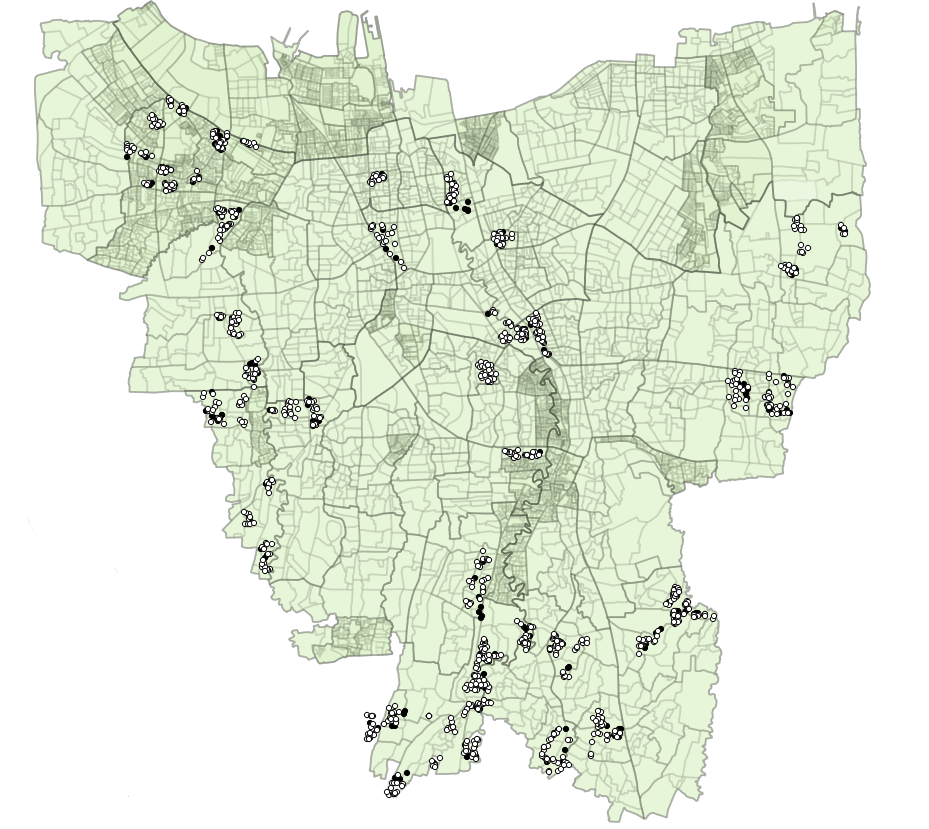
\includegraphics[width=120mm]{FigmapTC.png}
\end{figure}


\begin{figure}[h!]
    \centering
    \caption{Treatment Distribution across Retailers: Village Pegangsaan}
   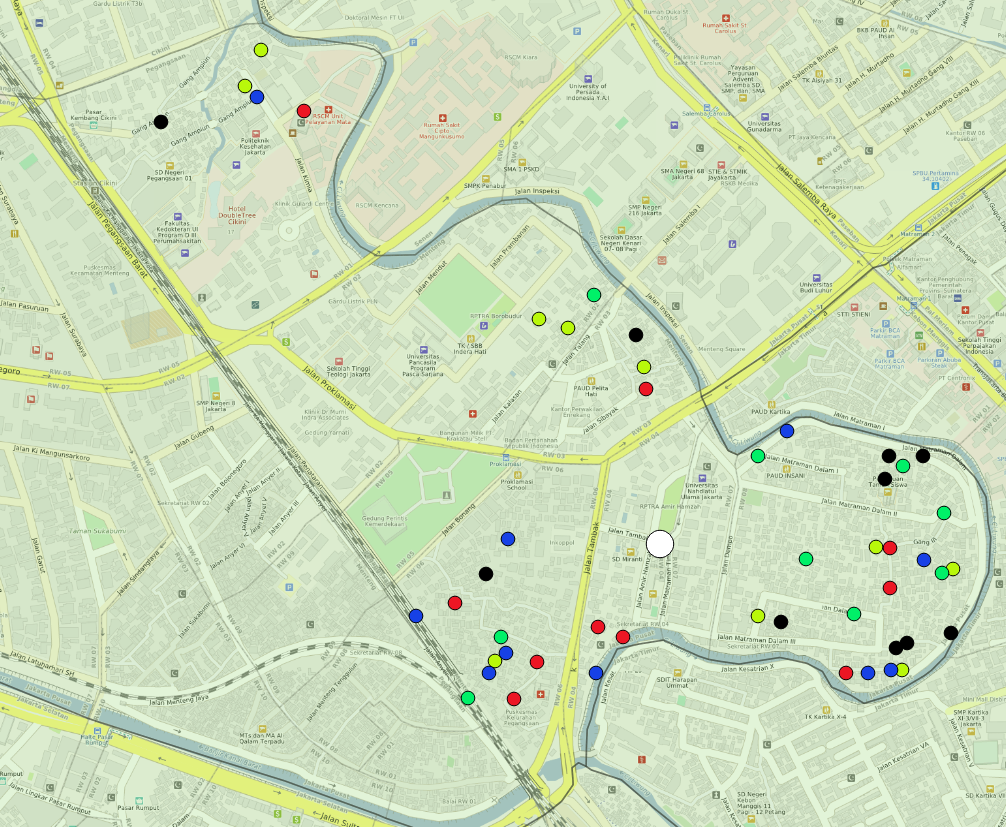
\includegraphics[width=120mm]{FigmapZoom.png}
\end{figure}


\pagebreak

\begin{figure}[h!]
    \centering
    \caption{Movie Screening Locations (big white) and Firms invited to the movie}
   	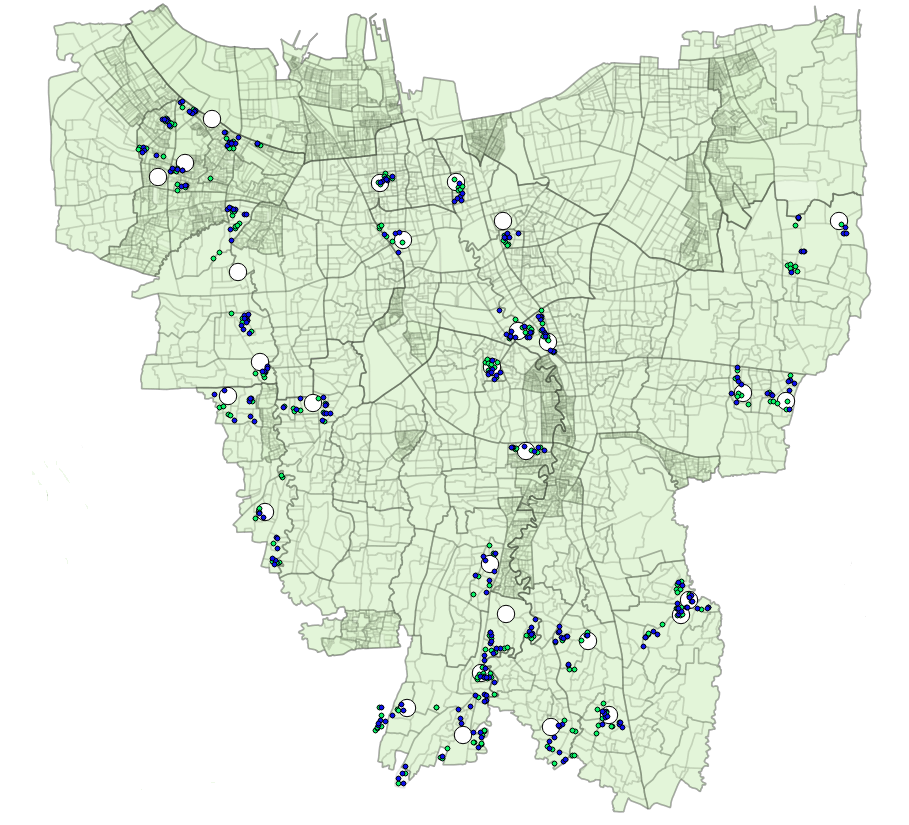
\includegraphics[width=120mm]{FigmapMovie.png}
\end{figure}

\end{landscape}
\pagebreak


\section{Sampling Protocol} \label{sec:appendixd}
\begin{enumerate}

	\item In the order given by the randomized list of selected villages, move 					into a village by approaching the respective head of the village.

	\item Obtain a list of all communities within the respective village and their 				boundaries.
	
	\item Generate a second list that contains these communities in random order.

	\item Move into a village according to the randomized list and, within each 				village, approach the owner of every shop that satisfies the following 				criteria:

	\begin{enumerate}
	
		\item The shop is at a distance of at least 30 meters to any other shop 					already listed.

		\item The shop is not a mere handcart or not otherwise easily moved.

		\item The shop is at least 4 $m^2$ in size

		\item The shop offers products from at least 2 product categories out of 					the following list:

		\begin{enumerate}


			\item Perishables (vegetables, fruits, eggs, rice, etc.)
			\item Pre-packaged food
			\item Soft-drinks and packaged drinks
			\item Snacks
			\item Tobacco
			\item Medicine
			\item Cleaning products
			\item Personal care
			\item DIY products

		\end{enumerate}

		\item The shop owner professes an aspiration to grow their business.

	\end{enumerate}

	\item Conditional upon the shop owner consenting, conduct the interview.

	\item Within the respective community, continue interviewing the owners of all 				shops that satisfy above mentioned criteria.

	\item If at any time the number of shops interviewed within the respective 					village equals or exceeds 67, continue interviewing all shops within 				the communities already moved into, but do not begin sampling in any 				new community within that village.

	\item If and when the total number of shops interviewed equals or exceeds 					2000, continue interviewing all shops within the village until the 					number of shops interviewed within the respective village equals or 				exceeds 67, in which case you continue interviewing all shops within 				the communities already moved into, but do not move into any new 					community within that village (just as outlined above).

\end{enumerate}
\pagebreak
\section{Project Timeline} \label{sec.timeline}

\begin{figure}[h]
    \centering
    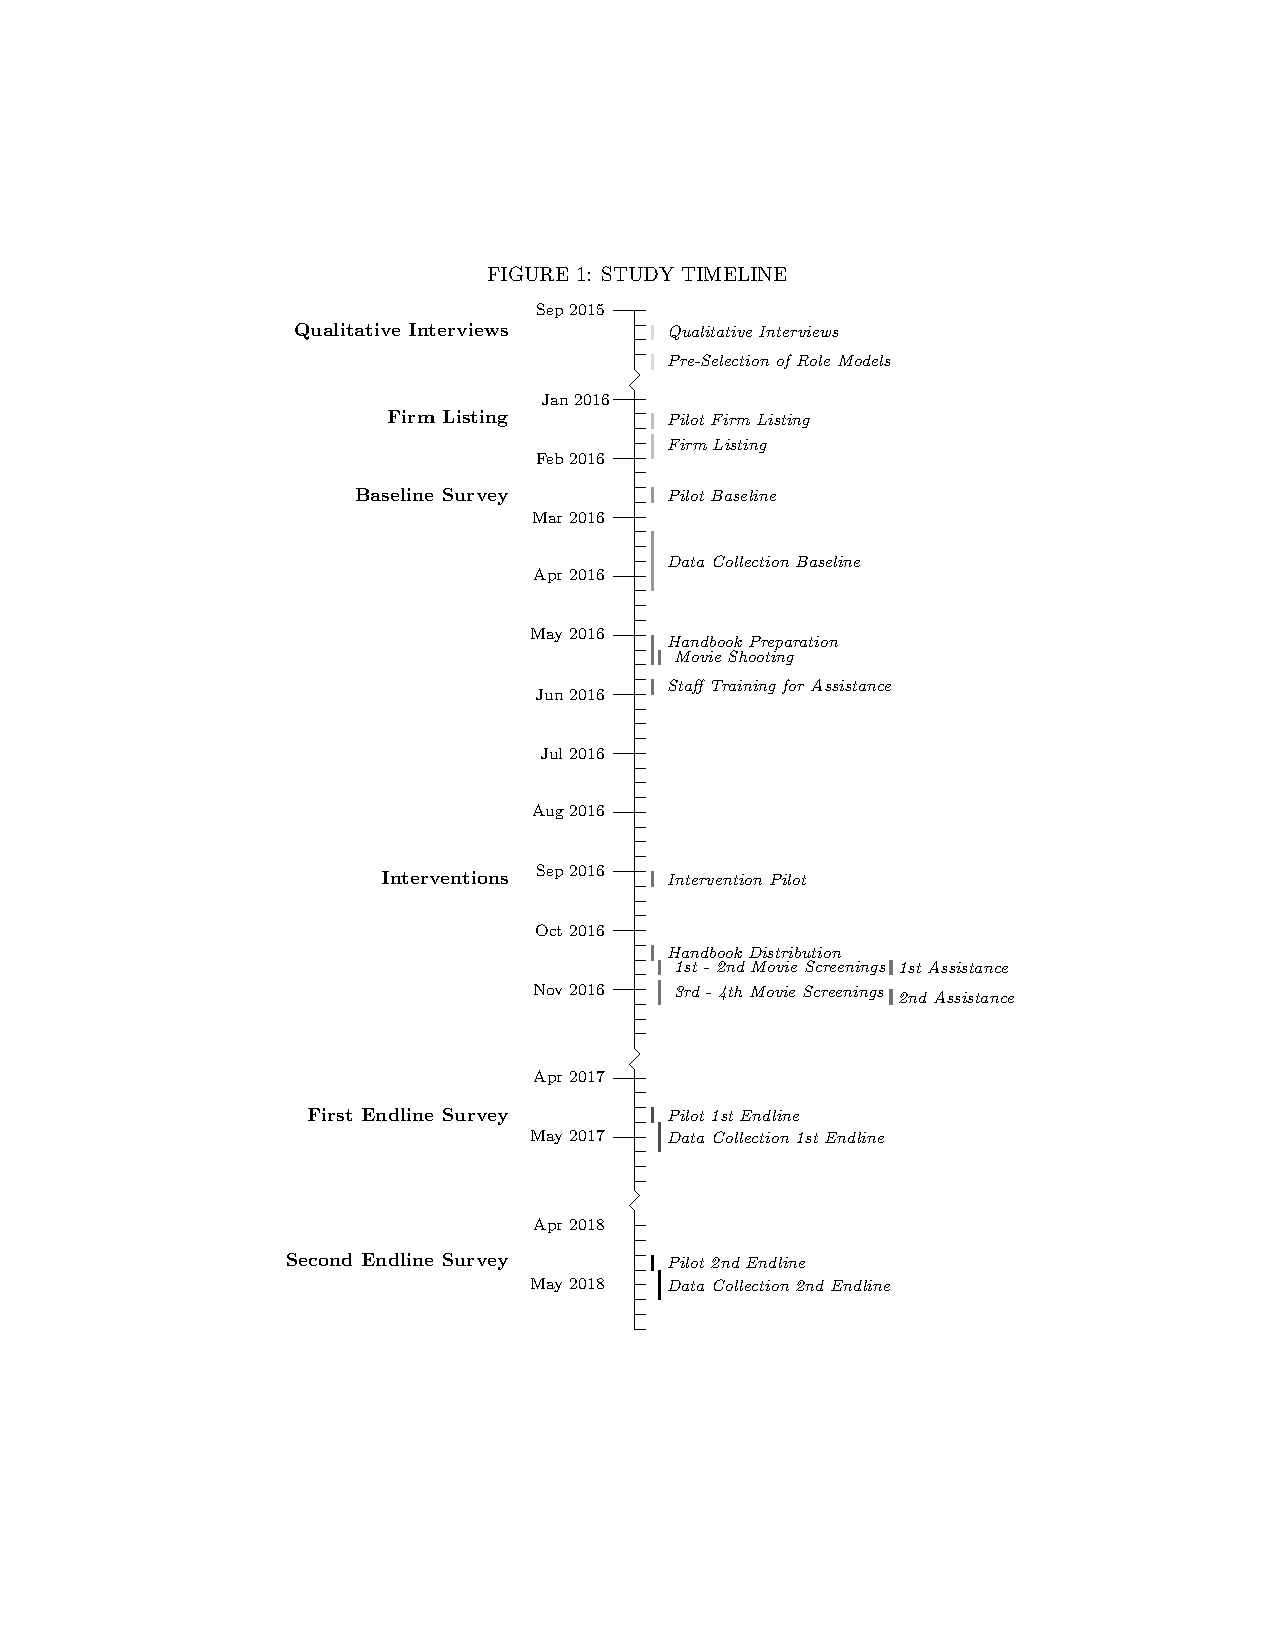
\includepdf[pages=-]{FigTimeline.pdf}
\end{figure}

\pagebreak
\section{Experimental Design} \label{sec:design}

\begin{table}[h!]
  \centering
  \renewcommand{\arraystretch}{1.4}
  \begin{tabular}{|c|c|c|c|c|c|c|c|c|}
    \hline
    \multicolumn{9}{|c|}{\textbf{Total Sample}}\\
    \multicolumn{9}{|c|}{1301 firms}\\
    \hline
    \multicolumn{1}{|c}{\textbf{Control}} & \multicolumn{8}{|c|}{\textbf{Handbooks}}\\
    \multicolumn{1}{|c}{261 firms} & \multicolumn{8}{|c|}{1040 firms}\\
    \cline{2-9}
    \multicolumn{1}{|c}{} & \multicolumn{8}{|c|}{\textbf{Returns to Adoption Framing}}\\
    \cline{2-9}
    \multicolumn{1}{|c}{} & \multicolumn{4}{|c}{\textit{Positive}} & \multicolumn{4}{|c|}{\textit{Negative}}\\
    \multicolumn{1}{|c}{} & \multicolumn{4}{|c}{520 firms} & \multicolumn{4}{|c|}{520 firms}\\
    \cline{2-9}
    \multicolumn{1}{|c}{} & \multicolumn{8}{|c|}{\textbf{Role-Model Movie}}\\
    \cline{2-9}
    \multicolumn{1}{|c}{} & \multicolumn{2}{|c}{\textit{Yes}} & \multicolumn{2}{|c}{\textit{No}} & \multicolumn{2}{|c}{\textit{Yes}} & \multicolumn{2}{|c|}{\textit{No}}\\
    \multicolumn{1}{|c}{} & \multicolumn{2}{|c}{260 firms} & \multicolumn{2}{|c}{260 firms} & \multicolumn{2}{|c}{260 firms} & \multicolumn{2}{|c|}{260 firms}\\
    \cline{2-9}
    \multicolumn{1}{|c}{} & \multicolumn{8}{|c|}{\textbf{Implementation Assistance}}\\
    \cline{2-9}
    \multicolumn{1}{|c}{} & \multicolumn{1}{|c}{\textit{Yes}} & \multicolumn{1}{|c}{\textit{No}} & \multicolumn{1}{|c}{\textit{Yes}} & \multicolumn{1}{|c}{\textit{No}} & \multicolumn{1}{|c}{\textit{Yes}} & \multicolumn{1}{|c}{\textit{No}} & \multicolumn{1}{|c}{\textit{Yes}} & \multicolumn{1}{|c|}{\textit{No}}\\
	\multicolumn{1}{|c}{} & \multicolumn{1}{|c}{130} & \multicolumn{1}{|c}{130} & \multicolumn{1}{|c}{130} & \multicolumn{1}{|c}{130} & \multicolumn{1}{|c}{130} & \multicolumn{1}{|c}{130} & \multicolumn{1}{|c}{130} & \multicolumn{1}{|c|}{130}\\
	\multicolumn{1}{|c}{} & \multicolumn{1}{|c}{firms} & \multicolumn{1}{|c}{firms} & \multicolumn{1}{|c}{firms} & \multicolumn{1}{|c}{firms} & \multicolumn{1}{|c}{firms} & \multicolumn{1}{|c}{firms} & \multicolumn{1}{|c}{firms} & \multicolumn{1}{|c|}{firms}\\
	\hline
  \end{tabular}
\end{table}



\pagebreak
%\section{Selection of Role Models}\label{sec:rolemodel}

%\pagebreak
%\section{Movie Script}\label{sec:movie}

%Available upon request.


\section{Businesses Pictures}\label{sec:expbusinesses}

\begin{figure}[h!]
\centering
\caption{Pictures of two shops representative of the sample of small-scale retail businesses in this study}
\label{warung1}
    \includegraphics[width=120mm]{Warung1.jpg}
\end{figure}

\begin{figure}[h!]
\centering
\label{warung2}
    \includegraphics[width=120mm]{Warung2.png}
\end{figure}

\end{appendices}
\end{document} 